\documentclass[12pt,a4paper]{article}

% Import basic packages first
\usepackage{tikz}
\usepackage{amsmath, amssymb}
\usepackage{geometry}
\usepackage{xcolor}
\usepackage{hyperref}

% Set page geometry
\geometry{margin=1in}

% Define colors
\definecolor{lightblue}{RGB}{173,216,230}
\definecolor{lightgreen}{RGB}{144,238,144}

% Title information
\title{\Large\textbf{Graph Theory Visualization}\\[0.5em]
       \normalsize A Visual Guide to Graph Theory Concepts}
\author{\textbf{Ashita Phulwani}\\
        Department of Mathematics}
\date{\today}

\begin{document}

% Title page
\maketitle

% Abstract or Introduction
\begin{abstract}
This document provides visual representations of fundamental graph theory concepts using TikZ. It includes examples of basic graphs, Euler paths, network flows, and spanning trees with detailed explanations.
\end{abstract}

\tableofcontents
\newpage

% First section with a simple example
\section{Basic Graph Concepts}

A graph consists of vertices (nodes) and edges connecting them. Here's a simple example:

\begin{center}
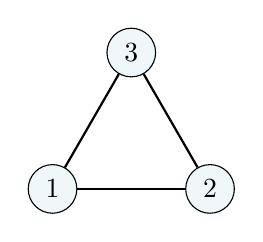
\begin{tikzpicture}
    % Create vertices
    \node[draw, circle, fill=lightblue!20] (A) at (0,0) {1};
    \node[draw, circle, fill=lightblue!20] (B) at (2,0) {2};
    \node[draw, circle, fill=lightblue!20] (C) at (1,1.732) {3};
    
    % Draw edges
    \draw[thick] (A) -- (B);
    \draw[thick] (B) -- (C);
    \draw[thick] (C) -- (A);
\end{tikzpicture}
\end{center}
This represents a simple triangle graph with three vertices and three edges.

\section{Euler Paths}

\begin{center}
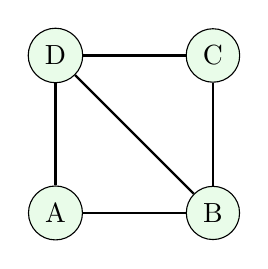
\begin{tikzpicture}
    \node[draw, circle, fill=lightgreen!20] (A) at (0,0) {A};
    \node[draw, circle, fill=lightgreen!20] (B) at (2,0) {B};
    \node[draw, circle, fill=lightgreen!20] (C) at (2,2) {C};
    \node[draw, circle, fill=lightgreen!20] (D) at (0,2) {D};
    
    \draw[thick] (A) -- (B);
    \draw[thick] (B) -- (C);
    \draw[thick] (C) -- (D);
    \draw[thick] (D) -- (A);
    \draw[thick] (B) -- (D);
\end{tikzpicture}
\end{center}

\section{Network Flow}

\begin{center}
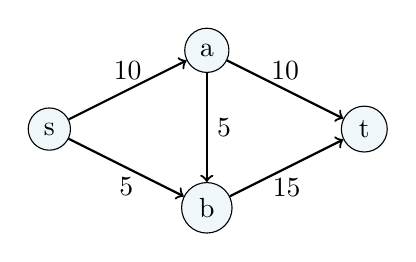
\begin{tikzpicture}
    \node[draw, circle, fill=lightblue!20] (s) at (0,1) {s};
    \node[draw, circle, fill=lightblue!20] (a) at (2,2) {a};
    \node[draw, circle, fill=lightblue!20] (b) at (2,0) {b};
    \node[draw, circle, fill=lightblue!20] (t) at (4,1) {t};
    
    \draw[->, thick] (s) -- node[above] {10} (a);
    \draw[->, thick] (a) -- node[right] {5} (b);
    \draw[->, thick] (b) -- node[below] {15} (t);
    \draw[->, thick] (s) -- node[below] {5} (b);
    \draw[->, thick] (a) -- node[above] {10} (t);
\end{tikzpicture}
\end{center}

\section{Spanning Trees}

\begin{center}
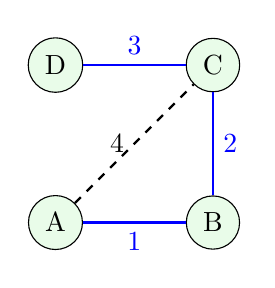
\begin{tikzpicture}
    \node[draw, circle, fill=lightgreen!20] (A) at (0,0) {A};
    \node[draw, circle, fill=lightgreen!20] (B) at (2,0) {B};
    \node[draw, circle, fill=lightgreen!20] (C) at (2,2) {C};
    \node[draw, circle, fill=lightgreen!20] (D) at (0,2) {D};
    
    \draw[thick, blue] (A) -- node[below] {1} (B);
    \draw[thick, blue] (B) -- node[right] {2} (C);
    \draw[thick, blue] (C) -- node[above] {3} (D);
    \draw[thick, dashed] (A) -- node[left] {4} (C);
\end{tikzpicture}
\end{center}

\section{Exercises}
\begin{enumerate}
    \item Find an Euler circuit in the first graph if one exists.
    \item Calculate the maximum flow in the network diagram.
    \item Identify the minimum spanning tree in the last graph.
\end{enumerate}

\end{document}